\begin{enumerate}[label=\thesubsection.\arabic*.,ref=\thesubsection.\theenumi]

\numberwithin{equation}{enumi}
\numberwithin{figure}{enumi}

\item For a particular amplifier connected in a feedback loop in which the output voltage is sampled,measurement of the output resistance before and after the loop is connected shows a change by a factor of 100.Is the resistance with feedback higher or lower?What is the value of the loop gain GH? If $R_{of}$ is 100 $\Omega$ ,what is $R_o$ without feedback.

\solution
We know that,
\begin{align}
    R_o = R_{of}(1+GH)
    \label{eq:ee18btech11042_1}
\end{align}
Output resistance before and after the loop is connected changes bya factor 100.So,

\begin{align}
    GH =99
\end{align}
Open loop gain GH is  99.
\newline
Given,
\begin{align}
    R_{of} = 100 
    \label{eq:ee18btech11042_3}
\end{align}
\begin{align}
    R_o = 100(1+99)
    \label{eq:ee18btech11042_4}
\end{align}
\begin{align}
    R_o = 10000
    \label{eq:ee18btech11042_5}
\end{align}
Output resistance without feedback  is   10k$\Omega$
\newline
Output resistance without feedback is greater than with feedback.
\item
The following code generates the values
\begin{lstlisting}
codes/ee18btech11042.py
\end{lstlisting}

\item Design a circuit.
\solution


\begin{figure}[!h]
		\resizebox{\columnwidth}{!}{\begin{circuitikz}[american]


    \ctikzset{tripoles/mos style/arrows}
    \draw(0,0)to [resistor, l = $R_S$] (1,0)--(3,0);
    \draw(3,0)--(4,0)--(4,-0.5) to [resistor, l = $R_{id}$,v> = $V_1$](4,-1.5)--(4,-2.5);
    
    \draw(4,-2.5)--(1,-2.5)--(1,-4)--(1,-8)--(1,-9)to [resistor,l = $R_1$] (1,-10);
    \draw(1,-10) node[ground]{};
    \draw(0,0)--(-2,0) to [V,l = $V_s$] (-2,-4);
    \draw(-2,-4) node[ground]{};
    \draw(1,-8)--(3,-8) to [resistor,l = $R_2$] (5,-8)-- (9,-8)--(9,-1.5);
    \draw(9,-1.5)--(10,-1.5)--(10,-2) to [resistor,l = $R_L$](10,-3) --(10,-4);
    \draw(10,-4)node[ground]{};
    \draw(4,-1.5) to [open,](7,-1.5);
    \draw(7,-1.5)--(7.5,-1.5) to [resistor,l = $r_o$](8.5,-1.5);
    \draw(8.5,-1.5)--(9,-1.5);
    \draw(7,-1.5)--(7,-2) to [cV,l = $\mu V_1$](7,-2.75)--(7,-3.25);
    \draw (7,-3.25)node[ground]{};
    \draw(8.75,-1.5)--(3,-5.75)--(3,1.5)--(8.75,-1.5);
    \draw(10,-1.5) node[circle,fill,inner sep = 2pt ,label = right:$V_o$]{};
    \end{circuitikz}}
\caption{Amplifier Circuit}
\label{fig:ee18btech11042_1}
\end{figure}
Feedback Gain
\begin{align}
    H = \frac{R_1}{R_1+R_2} = \frac{1}{40}
    \label{eq:ee18btech11042_6}
\end{align}
\begin{figure}[!h]
		\resizebox{\columnwidth}{!}{\begin{circuitikz}[american]
    
    \ctikzset{tripoles/mos style/arrows}
    \draw(0,0) to [resistor,l = $R_s$] (2,0) --(3,0)--(3,-1) to [resistor,l = $R_{id}$,v>=$V_1$](3,-3);
    \draw (3,-3) to [resistor,l = $R_1//R_2$] (0,-3);
    \draw(0,0) to [open,v>=$V_f$](0,-3);
    \draw(3,0) to [open] (4,0);
    \draw (4,0)--(5,0) to [resistor,l = $ r_o$] (6,0)--(6.5,0);
    \draw(6.5,0) to [resistor,l = $R_1+R_2$](6.5,-3);
    \draw(6.5,-3) node [ground]{};
    \draw(6.5,0)--(8.5,0)to [resistor,l = $R_L$] (8.5,-3);
    \draw(8.5,-3)node [ground]{};
    \draw(4,0)to [cV,l = $\mu V_1$] (4,-3);
    \draw(4,-3) node[ground]{};
    \draw(8.5,0)node[circle,fill,inner sep = 2pt,label = $V_o$]{};
    \end{circuitikz}
 }
\caption{H circuit}
\label{fig:ee18btech11042_2}
\end{figure}
From fig \ref{fig:ee18btech11042_2},
Open Loop  input resistance
\begin{align}
    R_{in} = R_s+R_{id}+(R_1//R_2)
    \label{eq:ee18btech11042_7}
\end{align}
Open loop output resistance 
\begin{align}
    R_o = r_o//R_L//(R_1+R_2)
    \label{eq:ee18btech11042_8}
\end{align}
Open Loop gain
\begin{align}
    G = \mu \frac{R_{id}}{R_s+R_{id}+(R_1//R_2)}\frac{R_L//R_1+R_2}{(r_o+(R_L//R_1+R_2))}
    \label{eq:ee18btech11042_9}
\end{align}
\begin{table}[!h]
    \centering
  	\resizebox{\columnwidth}{!}{\input{./table/ee18btech11042/table.tex}}
    \caption{parameter values}
    \label{table:ee18btech11042_1}
\end{table}

 Closed Loop Gain   $\frac{G}{1+GH}$  is 39.6


\item Verify through spice.
\newline
The following file provides how to simulate the spice file.
\begin{lstlisting}
spice/ee18btech11042/readme
\end{lstlisting}


 The following is .net list file for spice simulation
 
\begin{lstlisting}
spice/ee18btech11042/ee18btech11042.net
\end{lstlisting}
Given,
\begin{align}
    V_s (t)= sin(2000\pi t)
    \label{eq:ee18btech11042_11}
\end{align}
We got output as
\begin{align}
    V_o(t) = 40 sin(2000\pi t)
    \label{eq:ee18btech11042_12}
\end{align}
Overall gain  $\frac{V_o(t)}{V_{in}(t)}$ is 40 same as thereotical value.
\begin{figure}[!ht]
    
    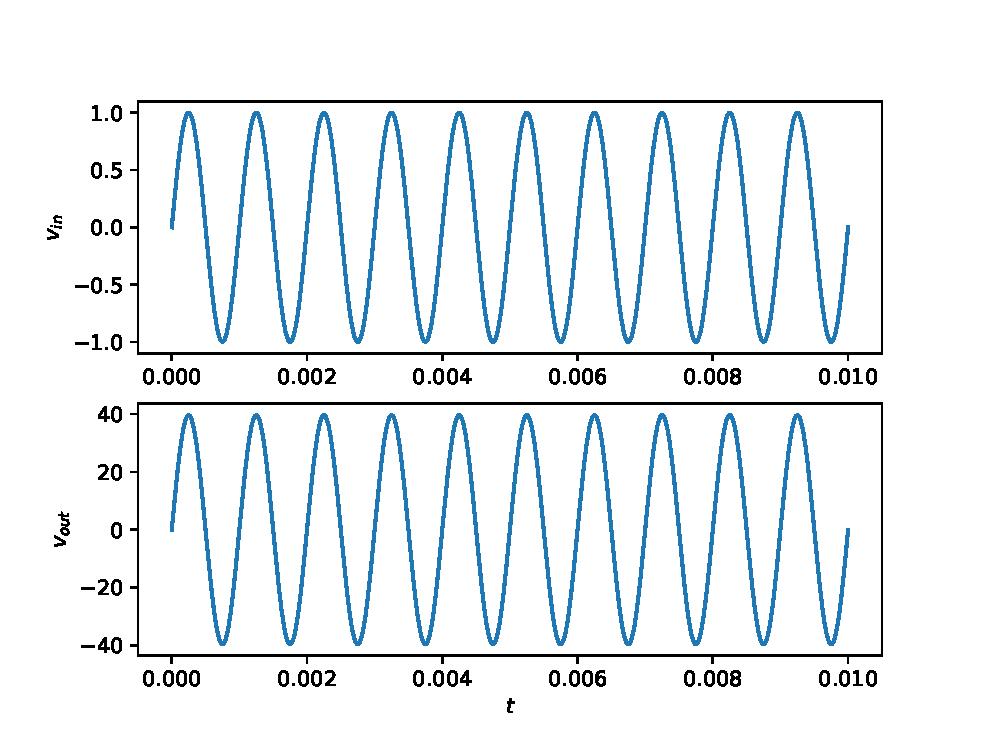
\includegraphics[width = \columnwidth]{./spice/ee18btech11042/spice.eps}
    \caption{Time response of system}
    \label{fig:ee18btech11042_3}
\end{figure}
The following code creates the python plots.
\begin{lstlisting}
spice/ee18btech11042/ee18btech11042_spice.py
\end{lstlisting}







\end{enumerate}



